\chapter{Sample Computers}
\label{c-samples}

\section{32 Bit Pipelined Computer}
Consider a 32 bit pipelined computer with a 1.0 GHz clock and an ISA that has three categories of commands:

\begin{tabular}{|c|c|} \hline
          & Freq \\ \hline
  Branch  & .2   \\ \hline
  Memory  & .3   \\ \hline
  Other   & .5   \\ \hline
\end{tabular}

The computer has a 64 bit memory bus that operates at 500 MHz.  The bus requires that requests and responses take 1 cycle.  The memory takes 40ns to respond to a request and can do burst sends with a delay of 10ns.  The bus requires 3 cycles to initiate a request and 2 cycles to transmit the response.  The bus is DMA and requires 710 CPU cycles to set up a transfer, 275 cycles to complete, 500 cycles to handle errors (1\% of the time).

The machine has two disks that have a combined transfer rate of 20MB/s, and a total latency of 6.8 ms.  The computer has virtual memory with a page size of 64KB.

\begin{enumerate}
\item What is the bandwidth of the bus?

{\color{ans}

We have been assuming the installed RAM to be integral in the bus design, so the answer would be:

\beqn
\hbox{Bandwidth} & = & \frac{\hbox{Data Transferred}}{\hbox{Time of Transfer}} \\
 & = & \frac{\hbox{Data Transferred}}{\hbox{Number of Cycles}\times\hbox{Time of 1 Cycle}} \\
 & = & \frac{\hbox{Data Transferred}\times\hbox{Bus Clock Frequency}}{\hbox{Cycles to Initiate}+\hbox{Cycles to Respond}+\hbox{Cycles to Get Data}} \\
 & = & \frac{8 \hbox{Bytes}\times 500 \hbox{MHz}}{3+2+(40\hbox{ns}\times 500\hbox{MHz})} \\
 & = & \frac{4000\hbox{MB/s}}{25} \\
 & = & 160\hbox{MB/s}
\eeqn

You might have noted that be RAM supports a burst transfer mode.  As the size of the burst increases the effective time to get the data approaches the burst time of 10 ns (down from 40 ns).  If you assumed this you would have found the bandwidth to be 400 MB/s.
}

\item If the computer had to continually page, how much of the CPU's time and the bus's bandwidth would it use?

{\color{ans}
Note that in memory KB = $2^{10}$ bytes, but in networks KB = $10^3$ bytes.  As they are similar, we will ignore the difference as the book does.  Additionally, we will assume the pages are spread across both disks so as to maximize the transfer.

The time it takes to transfer one page is given by:
\beqn
T_{\hbox{transfer}} & = & \hbox{time to get the data} + \hbox{time to send the data} \\
&=& \hbox{total latency} + \frac{\hbox{Data Sent}}{\hbox{Transmission Rate}} \\
&=& 6.8\hbox{ms}+ \frac{64\hbox{KB}}{20\hbox{MB/s}} \\
&=& 6.8\hbox{ms}+3.2\hbox{ms} \\
&=& 10\hbox{ms}.
\eeqn

The data rate for the transfer is:
\beqn
R_{\hbox{Data}} &=& \frac{\hbox{Data Sent}}{T_{\hbox{transfer}}} \\
&=& \frac{64\hbox{KB}}{10\hbox{ms}} \\
&=& 6.4\hbox{MB/s}.
\eeqn

Using the figure of 160 MB/s for the bus's bandwidth we find:
\beqn
\hbox{Percent Utilization of Bus} &=& \frac{\hbox{Bandwidth Used}}{\hbox{Bandwidth Available}}\times 100\hbox{\%} \\
&=& \frac{6.4 \hbox{MB/s}}{160 \hbox{MB/s}}\times 100\hbox{\%} \\
&=& 4\hbox{\%}.
\eeqn

Now let's look at the impact on the CPU.  We need to find the number of cycles the CPU must use to handle the transfer.
\beqn
\hbox{Cycles Per Transfer}
&=& \frac{\hbox{Cycles to Set Up}+\hbox{Cycles to Finish}+\hbox{error rate}\times\hbox{Cycle to Handle Errors}}{1-\hbox{error rate}} \\
&=& \frac{710+275+.01\times 500}{1-.01} \\
&=& \frac{990}{.99} \\
&=& 1000
\eeqn

The utilization of the CPU is thus:
\beqn
\hbox{Percent Utilization of CPU}
&=& \frac{\frac{\hbox{Cycles Per Transfer}}{T_{\hbox{transfer}}}}{\hbox{CPU Clock Frequency}}\times 100\hbox{\%} \\
&=& \frac{\frac{1000}{10\hbox{ms}}}{1\hbox{GHz}}\times 100\hbox{\%} \\
&=& 0.01\hbox{\%}
\eeqn

Thus we have a negligible impact.

}

\item What block size of the cache would cause the least impact on the CPI of the computer due to misses, assuming the instruction and data miss rate are equal?

\begin{tabular}{|l|cccc|} \hline
Block Size      & 2 words & 4 words & 8 words & 16 words \\ \hline
Miss Rate       & 4\%     & 2\%     & 1.2\%   & 1\%      \\ \hline
\end{tabular}

{\color{ans}

The average increase to a command's CPI due to cache misses depends on if the command accesses memory just for the instruction fetch or also for the commands implementation.  We will therefor assess the impact to memory commands separate from branch and other commands.  The average increase for branch and other commands is given by:
\beqn
\Delta\hbox{CPI} &=& \hbox{miss rate}\times\hbox{Bus Cycles to Transfer}\times\frac{\hbox{CPU Clock Rate}}{\hbox{Bus Clock Rate}} \\
&=&\hbox{miss rate}\times\hbox{Bus Cycles to Transfer}\times 2.
\eeqn
The average impact for branch commands is twice the increase of branch and other commands.

The bus cycles to transfer $2N$ words is given by:
\beqn
\hbox{Cycle to Transfer} &=& \hbox{Cycles to Initiate}+\hbox{Cycles to Get First 2 Words} \\
& & \qquad +(N-1)\times\hbox{Cycle to Burst Get 2 Words} \\
& & \qquad + N\times\hbox{Cycles to Send 2 Words} \\
&=& 3+ (40\hbox{ns}\times 500\hbox{MHz})+(N-1)\times(10\hbox{ns}\times 500\hbox{MHz})+N\times 2 \\
&=& 18+7N
\eeqn

\begin{tabular}{|l|cc|} \hline
Block Size             & 2 words        & 4 words           \\ \hline
Miss Rate              & 4\%            & 2\%               \\ \hline
Bus Cycles to Transfer & 18+7(1)=25     & 18+7(2)=32        \\ \hline
$\Delta$CPI Not Memory & (.04)(25)(2)=2 & (.02)(32)(2)=1.28 \\ \hline
$\Delta$CPI Memory     & (2)(2)=4       & (2)(1.28)=2.56    \\ \hline
\end{tabular}

\begin{tabular}{|l|cc|} \hline
Block Size             & 8 words             & 16 words          \\ \hline
Miss Rate              & 1.2\%               & 1\%               \\ \hline
Bus Cycles to Transfer & 18+7(4)=46          & 18+7(8)=74        \\ \hline
$\Delta$CPI Not Memory & (.012)(46)(2)=1.104 & (.01)(74)(2)=1.48 \\ \hline
$\Delta$CPI Memory     & (2)(1.104)=2.208    & (2)(1.48)=2.96    \\ \hline
\end{tabular}

The least impact is given by a cache with blocks of 8 words in this case.

}


\item Design a dynamic branch predictor for the computer.

{\color{ans}

A good estimate of whether a branch will be taken is to remember whether it was taken last time.  Remembering if a branch was taken or not requires 1 bit per instruction tracked.  To keep the problem realistic we will add an additional 32-bit register.  Each bit in the register will indicate if the branch was taken for the last instruction whose address modulo 32 corresponds to the bit's location.  An easy way to implement this would be to take the outputs of the 32 bits and pass them into a $32\times 1$ MUX, whose address select lines are given the last five bits of the command's address (from PC for instance).  The branch taken signal could be sent from the control to the particular bit by using a $1\times 32$ DeMUX.

}


\item For this system, 60\% of the branch instructions make loops and the rest are for conditional execution.  On average, the code in a loop is executed 10 times.  What fraction of the time does your dynamic branch predictor, correctly predict the branch taken?

{\color{ans}

Loops occur 60\% of the time, conditional execution occurs 40\% of the time.  The dynamic branch selected above does not likely do anything for conditional execution branches, so it is most likely correct on 50\% of the conditional execution branch instructions.  In the loops, the method designed would be correct in all but the first and last execution of the loop, so 80\% on loops.

The net effect is $(.4)(.5)+(.6)(.8)=.68$ or 68\% of the time it is right.

}


\item Using the best cache and your dynamic branch predictor, calculate the average CPI and the performance of the computer in MIPS.

{\color{ans}

I forgot to give you base CPI and  the penalty to CPI for missing a branch. I wanted the base for all instructions to be 1 (ideal for piplined) and the penalty to be 3.  Sorry about that.

Average CPI is given by:
\beqn
\hbox{CPI}_{\hbox{avg}} &=& \sum_{i}(\hbox{CPI}_i\times \hbox{frequency}_i) \\
&=& \hbox{CPI}_{\hbox{Memory}}\times\hbox{freq}_{\hbox{Memory}} + \hbox{CPI}_{\hbox{Correct Branch}}\times\hbox{freq}_{\hbox{Correct Branch}} \\
& & \qquad +\hbox{CPI}_{\hbox{Incorrect Branch}}\times\hbox{freq}_{\hbox{Incorrect Branch}} + \hbox{CPI}_{\hbox{Other}}\times\hbox{freq}_{\hbox{Other}} \\
&=& (1+2.208)(.2)+(1+1.104)(.3\times .68) \\
& & \qquad +(1+1.104+3)(.3\times .32)+(1+1.104)(.5) \\
&=& 2.6128
\eeqn

MIPS is given by:
\beqn
\hbox{MIPS} &=& \frac{\hbox{CPU Clock Freq}}{\hbox{CPI}\times 10^6} \\
&=& \frac{10^9 \hbox{Cycles/s}}{2.6128\hbox{Cycle/Million Inst}\times 10^6} \\
&\approx & 383
\eeqn
}
\end{enumerate}



\section{One Command Computer}

Consider a computer which has only one command, subtract and branch if negative (SBrN D, S1, S2, Jump).  Which does:

\begin{verbatim}
D = S1 - S2
if D < 0 goto Jump
\end{verbatim}

Since there is only one command there is no need to include the opcode in the machine language instruction.  The system is to have 1K of memory divided into 256 words of 4 bytes each.  Since memory requires 1 bytes to specify the address of a memory location the instructions will have four fields of 1 byte each:

\begin{tabular}{|c|c|c|c|} \hline
Destination & Source 1 & Source 2 & Jump Address \\ \hline
\end{tabular}

\begin{enumerate}
    \item Design a CPU that implements this.

    {\color{ans}
    Sol:

    See Figure 1
    }

    \item Alter your design to make it a four stage pipeline with forwarding.

    {\color{ans}
    Sol:

    See Figure 2.  Note that the control to the forwarding MUXs can come from tag bits on the RAM (first idea) or comparators on the destination (better solution).
    }


\begin{figure}[h]
  % Requires \usepackage{graphicx}
  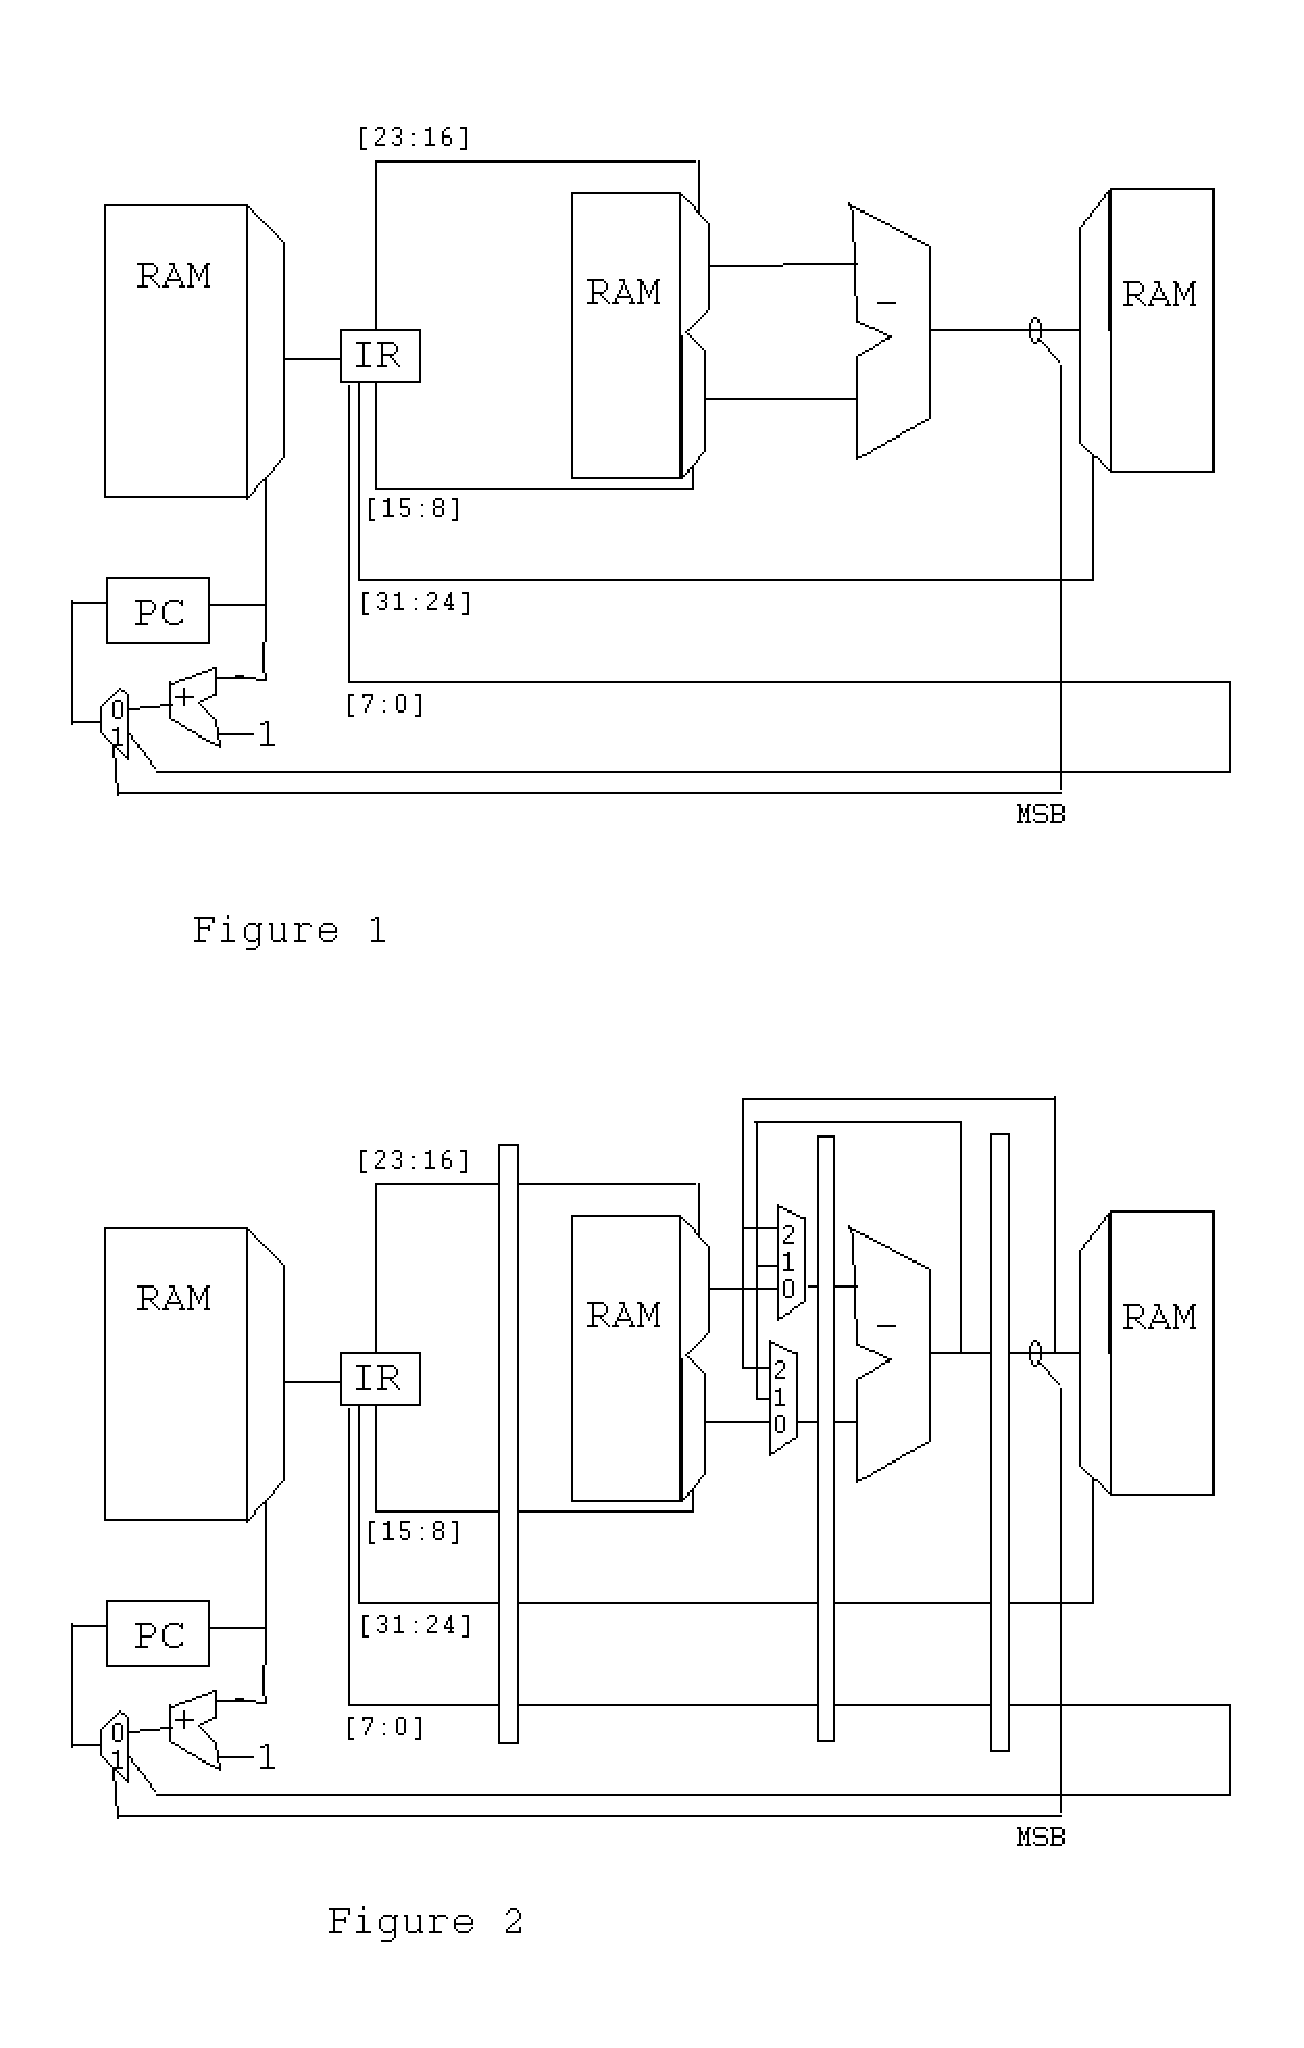
\includegraphics[width=5.25in]{kohw_one_inst_computer.eps}
  \caption{One Command Computer}\label{f-1command}
\end{figure}


    \item Design the control for the CPU (hardwired or microcoded)

    {\color{ans}
    Sol:

    In this case, most of the control signals are already handled.  All that remains undone is the load commands to the program counter and instruction register, and the read and write commands to memory.  The ifetch loop has only four states so the resulting logic table is:

\begin{tabular}{c||c|c|c|c}
$S_1 S_0$ & $S_1 S_0$ & Rpc & Rs1/Rs2 & Wd \\ \hline
00        & 01        & 1   & 0       & 0  \\
01        & 10        & 0   & 1       & 0  \\
10        & 11        & 0   & 0       & 0  \\
11        & 00        & 0   & 0       & 1  \\
\end{tabular}

Next $S_1 = S_1'\cdot S_0 + S_1\cdot S_0'$

Next $S_0 = S_0'$

$Rpc = S_1'\cdot S_0'$

$Rs1Rs2 = S_1'\cdot S_0$

$Wd = S_1\cdot S_0$
    }

    \item Show the tag bits (with their size), data field, and address of a 2-way associative write-back cache that uses NLLRU for this machine that has 8 locations.  How many total bits must be stored?

    {\color{ans}
    Sol:

    Main Memory has $2^8$ locations (n=8)

    Cache has $2^3$ locations (m=3)

    Associativity is $2^1$ (k=1)

    Each location in cache has a total of 42 bits
    \begin{enumerate}
        \item Address tag bits: n-(m-k) = 8-(3-1) = 6
        \item Valid tag bit: 1
        \item Dirty tag bit: 1
        \item NLLRU tag bits: 2 (the associativity)
        \item Data bits: 32
    \end{enumerate}

    The entire cache has $8\times 42 = 336$ bits

    }

    \item Show the cache accesses and calculate the hit ratio for the following memory values, assuming execution begins at location 0 and terminates when location 5 is reached.  If a location is not specified below, the contents are not important.  All values are in hex.

\begin{tabular}{l|c|c|c|c|cl|c|c|c|c|}
Address & D  & S1 & S2 & J  && Address & \multicolumn{4}{c|}{Data} \\ \cline{1-5} \cline{7-11}
00      & 87 & 88 & 80 & 01 && 80    & 00 & 00 & 00 & 00 \\
01      & 86 & 80 & 8B & 02 && 81    & FF & FF & FF & FF \\
02      & 87 & 87 & 86 & 03 && 82    & FF & FF & FF & FE \\
03      & 01 & 01 & 83 & 04 && 83    & 00 & 00 & 01 & 00 \\
04      & 82 & 82 & 81 & 01 &&       &    &    &    &    \\
\end{tabular}

    {\color{ans}
    Sol:

    (I have grouped my cache table so the associated portions of cache are on the same row.)

    Initial condition (hits=0, misses=0)

    \begin{tabular}{|c|c|c|c|c|c||c|c|c|c|c|c|} \hline
    NLLRU & V & D & Address & Loc & Data       & NLLRU & V & D & Address & Loc & Data        \\ \hline
    00    & 0 & 0 & 000000  & 000 & 0x00000000 & 00    & 0 & 0 & 000000  & 100 & 0x00000000  \\ \hline
    00    & 0 & 0 & 000000  & 001 & 0x00000000 & 00    & 0 & 0 & 000000  & 101 & 0x00000000  \\ \hline
    00    & 0 & 0 & 000000  & 010 & 0x00000000 & 00    & 0 & 0 & 000000  & 110 & 0x00000000  \\ \hline
    00    & 0 & 0 & 000000  & 011 & 0x00000000 & 00    & 0 & 0 & 000000  & 111 & 0x00000000  \\ \hline
    \end{tabular}


    command=0x87888001 (hits=0, misses=3) (read in 0 then 88, then 80 overwrote 0)

    \begin{tabular}{|c|c|c|c|c|c||c|c|c|c|c|c|} \hline
    NLLRU & V & D & Address & Loc & Data       & NLLRU & V & D & Address & Loc & Data        \\ \hline
    01    & 1 & 0 & 100000  & 000 & 0x00000000 & 00    & 1 & 0 & 100010  & 100 & 0x????????  \\ \hline
    00    & 0 & 0 & 000000  & 001 & 0x00000000 & 00    & 0 & 0 & 000000  & 101 & 0x00000000  \\ \hline
    00    & 0 & 0 & 000000  & 010 & 0x00000000 & 00    & 0 & 0 & 000000  & 110 & 0x00000000  \\ \hline
    01    & 1 & 1 & 100001  & 011 & 0x???????? & 00    & 0 & 0 & 000000  & 111 & 0x00000000  \\ \hline
    \end{tabular}


    command=0x86808B02 (hits=1, misses=5)

    \begin{tabular}{|c|c|c|c|c|c||c|c|c|c|c|c|} \hline
    LRU   & V & D & Address & Loc & Data       & LRU   & V & D & Address & Loc & Data        \\ \hline
    01    & 1 & 0 & 100000  & 000 & 0x00000000 & 00    & 1 & 0 & 100010  & 100 & 0x????????  \\ \hline
    01    & 1 & 0 & 000000  & 001 & 0x86808B02 & 00    & 0 & 0 & 000000  & 101 & 0x00000000  \\ \hline
    01    & 1 & 1 & 100001  & 010 & 0x???????? & 00    & 0 & 0 & 000000  & 110 & 0x00000000  \\ \hline
    00    & 1 & 1 & 100001  & 011 & 0x???????? & 10    & 1 & 0 & 100010  & 111 & 0x????????  \\ \hline
    \end{tabular}


    command=0x87878603 (hits=3, misses=6)

    \begin{tabular}{|c|c|c|c|c|c||c|c|c|c|c|c|} \hline
    LRU   & V & D & Address & Loc & Data       & LRU   & V & D & Address & Loc & Data        \\ \hline
    01    & 1 & 0 & 100000  & 000 & 0x00000000 & 00    & 1 & 0 & 100010  & 100 & 0x????????  \\ \hline
    01    & 1 & 0 & 000000  & 001 & 0x86808B02 & 00    & 0 & 0 & 000000  & 101 & 0x00000000  \\ \hline
    01    & 1 & 1 & 100001  & 010 & 0x???????? & 00    & 1 & 0 & 000000  & 110 & 0x87878603  \\ \hline
    01    & 1 & 1 & 100001  & 011 & 0x???????? & 00    & 1 & 0 & 100010  & 111 & 0x????????  \\ \hline
    \end{tabular}


    command=0x01018304 (hits=4, misses=8)

    \begin{tabular}{|c|c|c|c|c|c||c|c|c|c|c|c|} \hline
    LRU   & V & D & Address & Loc & Data       & LRU   & V & D & Address & Loc & Data        \\ \hline
    01    & 1 & 0 & 100000  & 000 & 0x00000000 & 00    & 1 & 0 & 100010  & 100 & 0x????????  \\ \hline
    01    & 1 & 1 & 000000  & 001 & 0x86808A02 & 00    & 0 & 0 & 000000  & 101 & 0x00000000  \\ \hline
    01    & 1 & 1 & 100001  & 010 & 0x???????? & 00    & 1 & 0 & 000000  & 110 & 0x87878603  \\ \hline
    01    & 1 & 1 & 100000  & 011 & 0x00000100 & 00    & 1 & 0 & 000000  & 111 & 0x01018304  \\ \hline
    \end{tabular}


    command=0x82828101 (hits=4, misses=11) (NOTE: 82 is 0xFFFFFFFF at end of command then jumps to 01)

    \begin{tabular}{|c|c|c|c|c|c||c|c|c|c|c|c|} \hline
    LRU   & V & D & Address & Loc & Data       & LRU   & V & D & Address & Loc & Data        \\ \hline
    00    & 1 & 0 & 100000  & 000 & 0x00000000 & 10    & 1 & 0 & 000001  & 100 & 0x82828101  \\ \hline
    00    & 1 & 1 & 000000  & 001 & 0x86808A02 & 10    & 1 & 0 & 100000  & 101 & 0xFFFFFFFF  \\ \hline
    00    & 1 & 1 & 100001  & 010 & 0x???????? & 10    & 1 & 0 & 100000  & 110 & 0xFFFFFFFF  \\ \hline
    01    & 1 & 1 & 100000  & 011 & 0x00000100 & 00    & 1 & 0 & 000000  & 111 & 0x01018304  \\ \hline
    \end{tabular}


    command=0x0x86808A02 (hits=6, misses=12)

    \begin{tabular}{|c|c|c|c|c|c||c|c|c|c|c|c|} \hline
    LRU   & V & D & Address & Loc & Data       & LRU   & V & D & Address & Loc & Data        \\ \hline
    00    & 1 & 0 & 100000  & 000 & 0x00000000 & 10    & 1 & 0 & 000001  & 100 & 0x82828101  \\ \hline
    01    & 1 & 1 & 000000  & 001 & 0x86808A02 & 00    & 1 & 0 & 100000  & 101 & 0xFFFFFFFF  \\ \hline
    00    & 1 & 1 & 100001  & 010 & 0x???????? & 10    & 1 & 0 & 100010  & 110 & 0x????????  \\ \hline
    01    & 1 & 1 & 100000  & 011 & 0x00000100 & 00    & 1 & 0 & 000000  & 111 & 0x01018304  \\ \hline
    \end{tabular}


    command=0x0x87878603 (hits=7, misses=14)

    \begin{tabular}{|c|c|c|c|c|c||c|c|c|c|c|c|} \hline
    LRU   & V & D & Address & Loc & Data       & LRU   & V & D & Address & Loc & Data        \\ \hline
    00    & 1 & 0 & 100000  & 000 & 0x00000000 & 10    & 1 & 0 & 000001  & 100 & 0x82828101  \\ \hline
    01    & 1 & 1 & 000000  & 001 & 0x86808A02 & 00    & 1 & 0 & 100000  & 101 & 0xFFFFFFFF  \\ \hline
    01    & 1 & 0 & 100001  & 010 & 0x87878603 & 00    & 1 & 0 & 100010  & 110 & 0x????????  \\ \hline
    00    & 1 & 1 & 100000  & 011 & 0x00000100 & 10    & 1 & 1 & 100001  & 111 & 0x????????  \\ \hline
    \end{tabular}


    command=0x0x01018304 (hits=8, misses=16)

    \begin{tabular}{|c|c|c|c|c|c||c|c|c|c|c|c|} \hline
    LRU   & V & D & Address & Loc & Data       & LRU   & V & D & Address & Loc & Data        \\ \hline
    00    & 1 & 0 & 100000  & 000 & 0x00000000 & 10    & 1 & 0 & 000001  & 100 & 0x82828101  \\ \hline
    01    & 1 & 1 & 000000  & 001 & 0x86808902 & 00    & 1 & 0 & 100000  & 101 & 0xFFFFFFFF  \\ \hline
    01    & 1 & 0 & 100001  & 010 & 0x87878603 & 00    & 1 & 0 & 100010  & 110 & 0x????????  \\ \hline
    01    & 1 & 0 & 000000  & 011 & 0x01018304 & 10    & 1 & 0 & 100003  & 111 & 0x00000100  \\ \hline
    \end{tabular}


    command=0x0x82828101 (hits=10, misses=17) (loaded 82 as 0xFFFFFFFF then -(-1) to get 0 which ends)

    \begin{tabular}{|c|c|c|c|c|c||c|c|c|c|c|c|} \hline
    LRU   & V & D & Address & Loc & Data       & LRU   & V & D & Address & Loc & Data        \\ \hline
    00    & 1 & 0 & 100000  & 000 & 0x00000000 & 10    & 1 & 0 & 000001  & 100 & 0x82828101  \\ \hline
    01    & 1 & 1 & 000000  & 001 & 0x86808902 & 00    & 1 & 0 & 100000  & 101 & 0xFFFFFFFF  \\ \hline
    00    & 1 & 0 & 100001  & 010 & 0x87878603 & 10    & 1 & 1 & 100000  & 110 & 0x00000000  \\ \hline
    01    & 1 & 0 & 000000  & 011 & 0x01018304 & 10    & 1 & 0 & 100003  & 111 & 0x00000100  \\ \hline
    \end{tabular}
    }


\item Assuming the cache has an access time of 4ns and the memory has an access time of 60ns, calculate the effective access time of the memory.

    {\color{ans}
    Sol:

    $hr=\frac{\hbox{hit}}{\hbox{hit}+\hbox{miss}}=\frac{10}{27}\approx .37$

    $mr=1-hr\approx 1-.37=.63$

    $T_{\hbox{eff}}=hr\times T_{\hbox{cache}}+mr\times T_{\hbox{RAM}}\approx .37\times 4 + .63\times 60 \approx 39 ns$
    }

\end{enumerate}

\section{Multiple Issue Machine}

You have a 1.5 GHz computer which can issue 2 instructions per cycle and a dynamic branch predictor that reduces the branch penalty from 4 cycles to 1 cycle, 90\% of the time.  Branch instructions are 15\% of all instructions, loads are 20\%, and stores are 5\%.

The cache is split into 4k instruction cache and 4k data cache.  The cache takes 2 ns to access.  The instruction cache has a block size of 2 words, has an associativity of 4, and a miss rate of 2\%.  The data cache has a block size of 4 words, an associativity of 2, is write-back, is not write-allocate, has a read miss rate of 5\%, a write miss rate of 2\%, and 10\% of the blocks are dirty.

The RAM is 8MB takes 50ns to access and can burst write subsequent accesses at 10ns.

  \begin{enumerate}
  \item How many cycles on average is the branch penalty?

  {\color{ans}
  \beqn
  Penalty_{branch}
  &=& f_{\hbox{pred. correct}}Cost_{\hbox{pred. correct}} + f_{\hbox{pred. error}}Cost_{\hbox{pred. error}} \\
  &=& .9\times 1 + .1\times 4 \\
  &=& 1.3
  \eeqn }

  \item How long does an instruction read miss take?

  {\color{ans} Two words have to be loaded on a miss, which takes 70ns. }

  \item How long does a data read miss take?

  {\color{ans} Four words have to be loaded on a miss, which takes 90ns.  Now 10\% of the time we also have to write four words, which takes the same as a read thus we have: $(1+.1)\times 90ns = 99ns$ }

  \item How long does a data write miss take?

  {\color{ans} On a write miss, four words have to be written, which takes 90ns. }

  \item What is the effective access time for instruction loads?

  {\color{ans}
  \beqn
  T_{Inst} &=& 2ns + .02\times 70ns \\
           &=& 3.4ns
  \eeqn}

  \item What is the effective access time for data reads?

  {\color{ans}
  \beqn
  T_{read} &=& 2ns + .05\times 99ns \\
           &=& 6.95ns
  \eeqn}

  \item What is the effective access time for data writes?

  {\color{ans}
  \beqn
  T_{write} &=& 2ns + .02\times 90ns \\
            &=& 3.8ns
  \eeqn}

  \item What is the CPI of this machine?

  {\color{ans}
  \beqn
  CPI &=& \frac{(1 + f_{branch}Penalty_{branch}+Penalty_{inst}+f_{read}\times Penalty_{read}+ f_{write}\times Penalty_{write})}{\hbox{\# inst per cycle}} \\
      &=& \frac{(1 + f_{branch}Penalty_{branch}+Clock_{rate}(T_{inst} + f_{read}\times T_{read}+ f_{write}\times T_{write}))}{\hbox{\# inst per cycle}} \\
      &=& \frac{1+.15\times 1.3 + 1.5 GHz(3.4ns+.2\times 6.95ns + .05\times 3.8ns)}{2} \\
      &=& 1.0830625
  \eeqn }

  \end{enumerate} 